\documentclass[12pt]{article}
\usepackage{graphicx} % Required for inserting images
\usepackage{fancyhdr} %para colocar um termo no final da página
\usepackage{amsmath}
\usepackage{graphicx}
\usepackage{cases}
\usepackage{listings}
\usepackage[dvipsnames]{xcolor}
\usepackage{xcolor}
\usepackage{amssymb}
\usepackage{epstopdf}
\epstopdfDeclareGraphicsRule
  {.gif}{png}{.png}{convert gif:\SourceFile.\SourceExt png:\OutputFile}
\AppendGraphicsExtensions{.gif}
\usepackage[colorlinks=true,linkcolor=blue,urlcolor=blue]{hyperref}

\lstdefinestyle{mystyle}{ 
    language =Python,
    backgroundcolor=\color{white},    
    commentstyle=\color{JungleGreen}, 
    keywordstyle=\color{BrickRed}, 
    morekeywords= \color{red},
    numberstyle=\tiny\color{lightgray}, 
    stringstyle=\color {blue}, 
    basicstyle=\ttfamily\footnotesize\bfseries, 
    breakatwhitespace=false,          
    breaklines=true,                  
    captionpos=t,                     
    keepspaces=true,                  
    numbers=left,                     
    numbersep=2pt,                   
    showspaces=false,                 
    showstringspaces=false, 
    showtabs=false,                   
    tabsize =1
}% -- Configurando o estilo personalizado: 
\lstset{style=mystyle}
% Reset page numbering and start from 1
\setlength{\headheight}{14.5pt}
\addtolength{\topmargin}{-2.5pt}
\pagestyle{fancy}
\newcommand\tab{\hspace{0.6cm}}
\title{\textbf{Relatório Parcial}}
\author{\\Caio Escórcio Lima Dourado \\NUSP: 13680313\and \\Victor Pedreira dos Santos Pepe\\NUSP: 13679565}
\date{26.03.2024}
\fancyhf{}
\fancyhead[C]{\thepage}

\cfoot{MAP3122 -- Cursos Coopeerativos -- 2024}
\renewcommand{\headrulewidth}{0pt}

\begin{document}
\begin{titlepage}
\centering
{\fontsize{24}{14}\selectfont \textbf{ Relatório Parcial} }\par
\vspace{0.4cm}
MAP3122 -- Cursos Cooperativos\par
{21.01.2024}\par
\vspace{1cm}

\includegraphics[width=0.9\textwidth]{minerva.jpeg}
\vspace{1cm}

\textbf{Caio Escórcio Lima Dourado}\par
NUSP: 13680313\par
\vspace{0.5cm}

\textbf{Victor Pedreira dos Santos Pepe}\par
NUSP: 13679565

\end{titlepage}
\newpage

\section{Introdução}
\hspace{0.6cm}Johannes Kepler, físico famoso pela elaboração das Leis de Kepler da Astronomia, como bem se sabe, dedicou a maior parte da sua vida ao estudo dos corpos celestes e de suas propriedades. Contudo, seja pela tecnologia da época ou até mesmo pela complexidade matemática que envolve o estudo dos astros, muitos de seus problemas  ficaram em aberto para as próximas gerações.\par
Um grande exemplo de problema não solucionado por Kepler é o Problema dos Dois Corpos, que envolvia a análise do movimento de planetas sujeitos aos campos gravitacionais um do outro. Tal problema, apesar de ter sido proposto e estudado pelo astrônomo em 1609, foi solucionado somente cerca de 78 anos depois, em 1687, graças outro tão famoso físico, Isaac Newton.\par
Assim, tomando como inspiração esse problema quase secular e a relação de movimento Terra-Sol-Lua, surgiu, por volta dos anos 1700, postulado pelo próprio Newton, uma nuance do que seria a ser Problema dos Três Corpos. À época, os objetivos de Newton foram apenas de tentar achar uma estabilidade de movimento entre os corpos do nosso sistema solar, o que não gerou muitas conclusões inovadoras ao considerarmos as suas outras contribuições para a matemática de sua época.\par
Contudo, com as novas leis físicas impostas por Newton, diversos cientistas do mundo inteiro, agora armados como o Cálculo e com as Leis de Newton, estavam dispostos a explorar as lacunas deixadas pelo físico, entre elas, o Problema dos Três Corpos. Assim, com o passar dos anos, tal desafio tornou-se mais e mais famoso no meios científicos, passando pelas mãos de matemáticos como D'Alembert e Poincaré, até chegar à proposição que temos hoje.\par
Fato é, esse problema se perpetuou desde o início da teoria gravitacional até os dias de hoje e, afirmativamente, é objeto de estudo de diversas áreas matemáticas, como busca-se mostrar neste documento.
\newpage
\section{Modelagem Matemática}
\hspace{0.6cm}O Problema dos Três Corpos (\textit{Three-Body Problem}, TBP) atualmente envolve diversas áreas matemática, como Equações Diferenciais, Geometria Euclidiana e até mesmo Caos. Sua proposição mais famosa consiste em um sistema de 3 corpos de mesma massa, esféricos e pontuais, localizados nos vértices de um triângulo pitagórico com lados de 3, de 4 e de 5 unidades arbitrariamente grandes quando comparadas ao raio dos corpos -- \textit{condições iniciais} do sistema -- que são atraídos gravitacionalmente uns pelos outros seguindo a Lei de Newton para Gravitação:\par
\vspace{0.4cm}

\begin{equation*}
\overrightarrow{F} = -{\frac{G\cdot m_1\cdot m_2}{r^2}\cdot \hat{r}}
\end{equation*}
\vspace{0.4cm}

onde:
\vspace{0.4cm}

\begin{itemize}
\item G é uma constante;
\item r é a distância entre os planetas;
\item m1 e m2 são as massas dos planetas 1 e 2, respectivamente;
\end{itemize}\vspace{1cm}
\hspace{0.6cm}Assim, uma vez que:
\vspace{0.4cm}

\begin{equation*}
    \overrightarrow{F_x} = m_x\ddot{r_x}\cdot \hat{r_x}
\end{equation*}
\vspace{0.4cm}

E, levando em consideração o plano vetorial bidimensional em que os corpos se encontram, bem como a interação gravitacional par a par temos os seguinte sistema diferencial:
\vspace{0.4cm}

\begin{equation*}
    \begin{cases}
       \ddot{\overrightarrow{r_1}} = -Gm_2\frac{\overrightarrow{r_1}-\overrightarrow{r_2}}{|\overrightarrow{r_1}-\overrightarrow{r_2}|^3} -Gm_3\frac{\overrightarrow{r_1}-\overrightarrow{r_3}}{\left|\overrightarrow{r_1}-\overrightarrow{r_3}\right|^3} \\
       \\
      \ddot{\overrightarrow{r_2}} = -Gm_1\frac{\overrightarrow{r_2}-\overrightarrow{r_1}}{|\overrightarrow{r_2}-\overrightarrow{r_1}|^3} -Gm_3\frac{\overrightarrow{r_2}-\overrightarrow{r_3}}{\left|\overrightarrow{r_2}-\overrightarrow{r_3}\right|^3}  \\
      \\
      \ddot{\overrightarrow{r_3}} = -Gm_1\frac{\overrightarrow{r_3}-\overrightarrow{r_1}}{|\overrightarrow{r_3}-\overrightarrow{r_1}|^3} -Gm_2\frac{\overrightarrow{r_3}-\overrightarrow{r_2}}{\left|\overrightarrow{r_3}-\overrightarrow{r_2}\right|^3}
      
    \end{cases}       
\end{equation*}

    \vspace{0.4cm}

Assim, a partir da análise de diversos trabalhos de pesquisa que envolvem o TBP, percebeu-se que, dependendo das condições iniciais escolhidas, a abordagem do problema tomaria configurações caóticas, fato que será descorrido em tópicos posteriores. Portanto, uma vez que o propósito deste relatório é essencialmente a análise de equações diferenciais a partir de métodos numéricos para compará-las com resultados previstos, optou-se por escolher uma configuração que obedecesse tal critério de previsibilidade. Então, definiu-se como condições iniciais uma configuração que, baseada em diversos estudos, tanto resultasse em um sistema harmônico (com orbitas controladas) quanto em uma figura conhecida e fácil de ser analisada: a configuração do infinito.
\vspace{0.4cm}
    
  \begin{equation*}
        \begin{cases}
        \overrightarrow{r_1}_{(0)} = (-0.97000436, 0.24308753, 0);\\
      
        \overrightarrow{r_2}_{(0)} = (0, 0, 0);\\
      
        \overrightarrow{r_3}_{(0)} = (0.97000436, -0.24308753, 0);
        \end{cases}
  \end{equation*}
    
      \vspace{0.4cm}
      
E:
\vspace{0.4cm}

\begin{equation*}
    m_1 = m_2 = m_3 = m = 1;
\end{equation*}
\vspace{0.4cm}

Para $\overrightarrow{r_1}$, $\overrightarrow{r_2}$ e $\overrightarrow{r_3}$ vetores do plano $\mathbb{R}^3$ com unidade de medida de distância arbitrária muito maiores que o raio esférico dos corpos -- a fim de garantir a sua característica pontual. Por sua vez, as massas $m_1$, $m_2$ e $m_3$ possuem todas massas escalares reais $m$, também em unidades arbitrárias, para garantir a proporcionalidade das forças e assim atender os critérios para evitar o caos.\par
Adicionalmente, tem-se que também atribuir condições iniciais nulas de velocidade ($\dot{\vec{r}}$) a fim de se ter puramente o movimento das forças gravitacionais, então:
\vspace{0.4cm}

    \begin{equation*}
    \begin{cases}
        \dot{\overrightarrow{r_1}}_{(0)} = (0.4662036850, 0.4323657300, 0)\\
        \dot{\overrightarrow{r_2}}_{(0)} = (-0.93240737, -0.86473146, 0)\\
        \dot{\overrightarrow{r_3}}_{(0)} = (0.4662036850, 0.4323657300, 0)\\
    \end{cases}
    \end{equation*}
    \vspace{0.4cm}
    
Em unidades arbitrárias de velocidade.
\vspace{0.4cm}

Finalmente, vale destacar que, apesar das massas serem todas iguais, a razão $m/G$, com $G$ a constante gravitacional, pode alterar a trajetoria dos planetas, uma vez que é o fato multiplicativo da aceleração dos corpos. Portanto, como última condição para o problema, definiu-se $G = 1$, na mesma ordem de grandeza das massas.

\begin{center}
    ------------------------------------------------------------------------------------------
\end{center}
\vspace{0.4cm}

Para adaptar o TBP para uma forma legível para discretização, são necessárias algumas tranformações de variáveis já que, essencialmente, esse problema contém configurações de EDO's de segunda ordem (acelerações). Transformações essas que, por comodidade, envolvem o seguinte modelo:
\vspace{0.4cm}

\begin{equation*}
    \ddot{y} = \frac{d\dot{y}}{dt} = \frac{d(f(y, t))}{dt} = F(y,t)
\end{equation*}

\begin{equation*}\rightarrow
\begin{cases}
        \dot{y} = h\\

        \dot{h} = F(y,t) \\
\end{cases}
\end{equation*}
\vspace{0.4cm}

Que aumenta o número de variáveis do sistema. Portanto, ao aplicar essa tranformação em cada um dos eixos x, y e z do $\mathbb{R}^3$ nos vetores que descrevem os movimentos dos corpos, temos:
\vspace{0.4cm}

\begin{equation*}
    \begin{cases}
        \dot{\overrightarrow{r_1}} = \overrightarrow{v_1}\\ 
        \dot{\overrightarrow{r_2}} = \overrightarrow{v_2}\\ 
        \dot{\overrightarrow{r_3}} = \overrightarrow{v_3}\\ \\
        \dot{\overrightarrow{v_1}} = -Gm_2\frac{\overrightarrow{r_1}-\overrightarrow{r_2}}{|\overrightarrow{r_1}-\overrightarrow{r_2}|^3} -Gm_3\frac{\overrightarrow{r_1}-\overrightarrow{r_3}}{\left|\overrightarrow{r_1}-\overrightarrow{r_3}\right|^3} \\
        \\
        \dot{\overrightarrow{v_2}} = -Gm_1\frac{\overrightarrow{r_2}-\overrightarrow{r_1}}{|\overrightarrow{r_2}-\overrightarrow{r_1}|^3} -Gm_3\frac{\overrightarrow{r_2}-\overrightarrow{r_3}}{\left|\overrightarrow{r_2}-\overrightarrow{r_3}\right|^3}  \\
        \\
        \dot{\overrightarrow{v_3}} = -Gm_1\frac{\overrightarrow{r_3}-\overrightarrow{r_1}}{|\overrightarrow{r_3}-\overrightarrow{r_1}|^3} -Gm_2\frac{\overrightarrow{r_3}-\overrightarrow{r_2}}{\left|\overrightarrow{r_3}-\overrightarrow{r_2}\right|^3}
    \end{cases}
\end{equation*}
\vspace{0.4cm}

Vale ressaltar que, apesar de todos os vetores possuírem dimensionalidade 3, o fato deles pertencerem inicalmente ao mesmo triângulo no plano $z=0$ e inexistirem forças externas atuando no eixo z do sistema -- vide 1ª lei de Newton -- pode-se considerar o sistema como bidimensional. 
 \newpage
 
 \section{Método de discretização}
 \subsection{Descrição do método}
 \hspace{0.6cm}Devido à natureza caótica do Problema dos Três Corpos, algumas observações devem ser feitas para que se possa calcular com melhor eficiência o desdobrar as EDO's -- vide o apêndice sobre Caos.\par
 Portanto, devido à quantidade de dados a serem processados durante o cálculo das posições dos corpos e a necessidade de precisão nessas medidas, optou-se por selecionar um método de discretização que ao mesmo tempo fosse simples, como também possuísse uma ordem de erro muito pequena: o Método de Runge-Kutta Clássico.\par
 Então, seguindo o estudo do método, dado um Problema de Cauchy, vetorialmente:
 \begin{equation*}
 \begin{cases}
          \dot{\overrightarrow{y}} = f(t, \overrightarrow{y})\\
          \overrightarrow{y}_{(t_0)} = \overrightarrow{y_0} 
 \end{cases}
 \end{equation*}

 Com $t \in I = [a, b]$. A discretização pelo Método de Runge-Kutta Clássico é dada por:

\begin{equation*}
          \overrightarrow{y}_{k+1} = \overrightarrow{y_k} + \overrightarrow{\Phi}(t_k, \Delta t, \overrightarrow{y_k})
\end{equation*}
\vspace{0.4cm}

para: 
\begin{equation*}
    \begin{cases}
          t_k = t_0 + k\Delta t\hspace{0.6cm}com\hspace{0.2cm} k \in \mathbb{N}: 0, ..., n\\
          \Delta t = \frac{b-a}{n}
    \end{cases}
\end{equation*}
\vspace{0.4cm}

 e, dados $\overrightarrow{K_1}$, ${\overrightarrow{K_2}}$, $\overrightarrow{K_3}$ e $\overrightarrow{K_4}$:
 \begin{equation*}
     \begin{cases}
         \overrightarrow{K_1} = \Delta tf(t_k, \overrightarrow{y_k})\\
         \overrightarrow{K_2} = \Delta tf(t_k + \frac{1}{2}\Delta t, \overrightarrow{y_k} + \frac{1}{2}\overrightarrow{K_1})\\
         \overrightarrow{K_3} = \Delta tf(t_k + \frac{1}{2}\Delta t, \overrightarrow{y_k} + \frac{1}{2}\overrightarrow{K_2})\\
         \overrightarrow{K_4} = \Delta tf(t_k + \Delta t, \overrightarrow{y_k} + \overrightarrow{K_3})
     \end{cases}
 \end{equation*}
 \vspace{0.4cm}

então:
 \begin{equation*}
     \begin{cases}
         \overrightarrow{y}_{k+1} = \overrightarrow{y_k} + \overrightarrow{\Phi}(t_k, \Delta t, \overrightarrow{y_k})\\
         \overrightarrow{\Phi}(t_k, \Delta t, \overrightarrow{y_k}) = \frac{1}{6}(\overrightarrow{K_1} + 2\overrightarrow{K_2} + 2\overrightarrow{K_3} + \overrightarrow{K_4})
     \end{cases}
 \end{equation*}
\vspace{0.4cm}

\hspace{0.6cm}Dessa forma, com esse método implícito, para utilizando as fórmulas para o cálculo do erro de discretização local, obtém-se que a ordem do erro é $O({\Delta t}^4)$, que será mostrada nas próximas seções, na Análise de Resultados.
 
 \newpage
 \subsection{Codificação do método}
 \hspace{0.6cm} Para implementar o algoritmo previamente descrito, optou-se por implementar uma abordagem orientada a objetos em Python(\textit{Object-Oriented Programming}), tomando como base do código a classe \textit{Planeta.py}:
 \vspace{0.4cm}
 
\begin{lstlisting}
import numpy as np

#Definicao de variaveis globais
G = 1 #fonte: https://pt.wikipedia.org/wiki/Constante_gravitacional_universal 6,6743xE-11

class Planeta:
    
    #Construtor do planeta   
    #Cada planeta possui posicao, massa e velocidade como caracteristicas instrinsecas
    def __init__ (self, posicao:np.array, massa:int, velocidade:np.array):
        self.posicao = posicao
        self.massa = massa
        self.velocidade = velocidade
        
    #Mede a distancia entre dois planetas (funcao estatica)
    def distancia (planeta_1, planeta_2):
        delta = planeta_1.posicao - planeta_2.posicao
        d = np.sqrt(delta.dot(delta)) #raiz do produto escalar entre duas distancias vetoriais
        
        return d #retorna a distancia escalar entre dois vetores
    
    def ac_rel (self, planeta_outro):
        ac = np.array([0, 0])
        if(np.any(self.posicao != planeta_outro.posicao)):
            ac = ((-1)*G*(planeta_outro.massa)*np.subtract(self.posicao, planeta_outro.posicao))/(Planeta.distancia(self, planeta_outro)**3) #ac_rel 1 para 2 = -G*(R_1 - R_2)/d^3
        return ac
 \end{lstlisting}
 
 \vspace{0.4cm}

 Nessa classe, definie-se um Planeta (corpo), com uma posição, uma massa e uma velocidade. Também implementou-se funções de cálculo de distâncias, que calcula a distância entre dois planetas usando os seus vetores de posição e uma função para calcular a aceleração relativa entre o planeta declarado e um outro planeta, utilizando a equação do $\dot{\overrightarrow{v}}$ da seção 2.\par
 
 Para o método de discretização, implementou-se uma classe \textit{Discretizacao.py}, para receber as condições iniciais dos planetas e retornar os pontos de suas trajetórias:\vspace{0.4cm}

 \begin{lstlisting}
import numpy as np
from Classes.Planeta import Planeta

massa = 1
G = 1

class Discretizacao:
    
    def __init__(self):
        pass
    
    #f(t, y) para o caso dos planetas
    def f(self, t, y): #y_k[i]
        #funcao para calcular a aceleracao
        a1 = lambda c1, c2, c3: c1.ac_rel(c2) + c1.ac_rel(c3)
        a2 = lambda c1, c2, c3: c2.ac_rel(c1) + c2.ac_rel(c3)
        a3 = lambda c1, c2, c3: c3.ac_rel(c2) + c3.ac_rel(c1)

        #Criando os planetas
        planeta_1 = Planeta(np.array([y[0], y[1]]), massa, np.array([y[6], y[7]]))
        planeta_2 = Planeta(np.array([y[2], y[3]]), massa, np.array([y[8], y[9]]))
        planeta_3 = Planeta(np.array([y[4], y[5]]), massa, np.array([y[10], y[11]]))

        #declara o vetor de retorno
        k = np.array([0.0, 0.0,
                      0.0, 0.0,
                      0.0, 0.0,
                      0.0, 0.0,
                      0.0, 0.0,
                      0.0, 0.0])

        #derivada da posicao = velocidade
        k[0], k[1] = planeta_1.velocidade[0], planeta_1.velocidade[1] 
        k[2], k[3] = planeta_2.velocidade[0], planeta_2.velocidade[1] 
        k[4], k[5] = planeta_3.velocidade[0], planeta_3.velocidade[1] 

        #derivada da velocidade = aceleracao
        k[6], k[7] = a1(planeta_1, planeta_2, planeta_3)
        k[8], k[9] = a2(planeta_1, planeta_2, planeta_3)
        k[10], k[11] = a3(planeta_1, planeta_2, planeta_3)

        return k

    #phi generico
    def phi(self, t, y, h):
        #declarando phi do Runge-Kutta
        #PLANETA
        # k_1 = h*self.f(t, y)
        # k_2 = h*self.f(t + h/2, y + k_1/2)
        # k_3 = h*self.f(t + h/2, y + k_2/2)
        # k_4 = h*self.f(t + h, y + k_3)
        
        #MANUFATURADA
        k_1 = h*self.f_manufaturada(t, y)
        k_2 = h*self.f_manufaturada(t + h/2, y + k_1/2)
        k_3 = h*self.f_manufaturada(t + h/2, y + k_2/2)
        k_4 = h*self.f_manufaturada(t + h, y + k_3)

        return (k_1 + 2*k_2 + 2*k_3 + k_4)/6

    def f_manufaturada(self, t, y): #f = y' ; y = e^(3t)*sin(5t) - 5; y(0) = -5
        return np.exp(3*t)*3*np.sin(5*t) + 5*np.exp(3*t)*np.cos(5*t)
    
    def exata_manufaturada(self, t):
        """y = e^(3t)*sin(5t) - 5"""
        return np.exp(3*t)*np.sin(5*t) - 5

    #metodo de discretizacao
    def calcula(self, n, intervalo_t, dim):
        #discretizacao do intervalo
        h = (intervalo_t[1] - intervalo_t[0])/n

        #inicializacao das variaveis
        i = 0
        #PLANETAS
        # t_k = np.zeros((30*n+1, 1))
        # y_k = np.zeros((30*n+1, dim))
        
        #MANUFATURA
        t_k = np.zeros((n+1, 1))
        y_k = np.zeros((n+1, dim))

        #inicializacao das condicoes iniciais
        t_k[0] = intervalo_t[0]
        #PLANETAS
        # y_k[0] = np.array([
        #     -0.97000436, 0.24308753,        #R_1: 0, 1
        #     0.97000436, -0.24308753,        #R_2: 2, 3
        #     0, 0,                           #R_3: 4, 5

        #     0.4662036850, 0.4323657300,     #V_1: 6, 7
        #     0.4662036850, 0.4323657300,     #V_2: 8, 9
        #     -0.93240737, -0.86473146        #V_3: 10, 11
        # ])  
        
        #MANUFATURA
        y_k[0] = np.array([-5])
        

        #loop para calcular os valores de y
        
        #PLANETA
        #for i in range(30*n):
        
        #Calculo da discretizacao
        for i in range(n):
            y_k[i+1] = y_k[i] + self.phi(t_k[i], y_k[i], h)
            t_k[i+1] = t_k[i] + h

        return y_k, t_k
    
    def converte(self, n):
        #y_k, t_k = self.calcula(100, [0, 1], 12)
        y_k, t_k = self.calcula(n, [0, 2], 1)
        i = 1
        #PLANETAS
        # pos1 = np.array([y_k[0][0], y_k[0][1]])
        # pos2 = np.array([y_k[0][2], y_k[0][3]])
        # pos3 = np.array([y_k[0][4], y_k[0][5]])
        # for i in range(30*n):
        #     pos1 = np.vstack([pos1, np.array([y_k[i][0], y_k[i][1]])])
        #     pos2 = np.vstack([pos2, np.array([y_k[i][2], y_k[i][3]])])
        #     pos3 = np.vstack([pos3, np.array([y_k[i][4], y_k[i][5]])])
        #return pos1, pos2, pos3
        
        #MANUFATURA
        return y_k, t_k
 \end{lstlisting}
 
\vspace{0.4cm}

Em uma breve leitura do código, podemos destacar 3 funções principais: \textit{phi()}, \textit{f()} ou \textit{$f_{manufaturada}$()} e \textit{calcula()}. Genericamente, cada função representa os passos do método de Runge-Kutta,  obedecendo necessariamente a ordem de operação descrito na seção de Descrição do Método. Vale ressaltar que o sistema foi montado para que, modificando adequadamente a função \textit{f()} e o vetor das condições iniciais \textit{$y_k$[0]}, é possível discretizar quaisquer problemas dados.\par

Para esclarecer o funcionamento das funções, podemos resumi-las da seguinte maneira:
\begin{itemize}
    \item phi(t, y, h): Recebe o vetor $y = y_k$, o instante $t = t_k$ e o incremento $h = \Delta t$ e calcular os $\kappa_1$, $\kappa_2$, $\kappa_3$ e $\kappa_4$ utilizando a função $f()$ ou $f_{manufaturada}$ e os argumentos da função. Ela retorna o incremento vetorial de $y_k$ para o cálculo de $y_{k+1}$\\
    \item f(t, y): Recebe o vetor $y = y_k$, o instante $t = t_k$ e, dependendo do problema proposto, pode ser modificada livremente para a discretização do problema. Ela retorna o que corresponderia a $\dot{\overrightarrow{y_k}}$ e é utilizada para o cáculos dos $\kappa$'s.\\
    \item calcula(n, $intervalo_t$, dim): recebe o número de passos $n$, o intervalo de discretização $intervalo_t$ e o inteiro $dim$ que indica a dimensão dos vetores de $y_k$ do problema. Vale ressaltar que o seu papel é simplesmente discretizar o intervalo de tempo, iniciar o vetor dos y's e realizar o \textit{loop} para o cálculo dos demais pontos da função utilizando phi(t, y, h) e f(t, y). Ela retorna os vetores finais de todos os $y_k$ e os $t_K$ do intervalo.
\end{itemize}

Finalmente, vale ressaltar o papel da função \textit{converte()}, que simplesmente gera os vetores de menor dimensão que serão plotados/utilizados para a verificação do método. Uma vez que o objetivo da disciplina não é necessariamente ensinar lógica de programação, o funcionamento a fundo do código não será explicado. Também recomenda-se uma breve leitura sobre o funcionamento da linguagem Python e da sua biblioteca NumPy para o entendimento completo do programa.
\newpage
\section{Modelagem polinomial dos resultados obtidos}
\hspace{0.6cm}A partir dos pontos gerados pelo algoritmo de Runge-Kutta multidimensional para o problema, utilizou-se os pontos obtidos para a modelagem da trajetória dos corpos via Spline Natural.
\vspace{0.4cm}

\subsection{Algoritmo de Spline Natural e resolução de sistemas lineares}
\hspace{0.6cm}Após a discretização do Problema dos 3 Corpos com o uso do Runge-Kutta Clássico, foram obtidos - para cada corpo - múltiplos  pares coordenados $(x,y)$, os quais descrevem a trajetória percorrida por eles. Com todos esses valores em mãos, é possível realizar uma modelagem polinomial por meio dos splines cúbicos. \par
Esse método numérico é muito utilizado quando se deseja aproximar (ou mesmo se obter) uma função desconhecida a partir de pontos conhecidos. A ideia básica dele é aproximar a função desconhecida utilizando múltiplos polinômios de terceiro grau, cada um deles abrangendo um sub-intervalo (todos de mesmo tamanho) da função. Quanto aos coeficientes dos polinômios, esses serão obtidos a partir da resolução de sistemas lineares, como veremos mais adiante.\par
Uma grande vantagem do uso dos splines cúbicos sobre outros métodos, como a interpolaçao de Lagrange, é que este último - principalmente quando se trata de problemas complexos e caóticos -  gera um polinômio de grau elevado, o qual pode flutuar de forma drástica, de modo que uma pequena flutuação localizada pode induzir flutuações grandes no intervalo inteiro. Já o método dos splines cúbicos, formado por múltiplos polinômios sucessivos que apresentam continuidade primeira e na segunda derivada, resulta numa forma mais suave. Um exemplo gráfico da aproximação por splines cúbicos pode ser visualizado na figura 1: 
\newpage


\begin{figure}
    \centering
    \includegraphics[width=0.9\textwidth]{splinecubico.png}
    \caption{Interpolação por splines cúbicos}
    \label{fig:enter-label}
\end{figure}



No problema abordado nesse relatório, foi possível obter uma série de pontos aproximados a partir da discretização de EDOs, mas não as funções que deram origem a elas, o que torna o uso dos splines extremamente conveniente na modelagem do problema dos 3 corpos. \par
Vale ressaltar que, como o problema é caótico, os polinômios obtidos a partir da resolução dos sistemas lineares de cada sistema será muito diferente dos demais para cada condição inicial selecionada.\par
Quanto ao método dos splines cúbicos, vamos supor que desejamos aproximar uma função $f(x)$ , da qual utilizaremos $n$ pontos igualmente espaçados no eixo $x$. Seja $ x = x_0, x_1, x_2, ... , x_n $ e $f(x) = f(x_0), f(x_1), f(x_2), ... , f(x_n)$ o conjunto de pontos coletados, temos que $h_0, h_1, h_2, ..., h_n{}_-{}_1$ são os intervalos entre duas abscissas consecutivas (ou seja, $h_k = x_k{}_+{}_1 - x_k{}$).  Além disso, denominamos $S(x)$ o polinômio completo para todo o intervalo $I$ no qual os $x_n$ pontos estão contidos. \par
Importante ressaltar também que iremos trabalhar com splines \textit{naturais}, ou seja, a segunda derivada de $S(x)$ é nula tanto no início quanto no final de $I$. Assim, temos:

\begin{equation*}
    \begin{cases}
    S(x) = S_j(x) = a_j + b_j(x - x_j) + c_j(x - x_j)^2 + d_j(x - x_j)^3,\hspace{0.3cm} x \in [x_j, x_j{}_+{}_1]\\
    S(x_j) = f(x_j), \hspace{0.3cm} j = 0, 1, 2, ..., n \\
    S_j{}_+{}_1(x_j{}_+{}_1) = S_j{}(x_j{}_+{}_1), \hspace{0.3cm} j = 0, 1, 2, ..., n-2 \\
     S'_j{}_+{}_1(x_j{}_+{}_1) = S'_j{}(x_j{}_+{}_1), \hspace{0.3cm} j = 0, 1, 2, ..., n-2 \\
      S''_j{}_+{}_1(x_j{}_+{}_1) = S''_j{}(x_j{}_+{}_1), \hspace{0.3cm} j = 0, 1, 2, ..., n-2 \\
      S''(x_0) = S''(x_n) = 0
    \end{cases}
\end{equation*}





 \vspace{0.4cm}
 Com todas as propriedades do spline natural descritas nas equações acima e  realizando algumas substituições, será possivel determinar os coeficientes dos polinômios a partir de um sistema linear. Inicialmente, tomemos $x = x_j{}_+{}_1$:


 \begin{numcases}{}
     S_j{}_+{}_1(x_j{}_+{}_1) = S_j{}(x_j{}_+{}_1) = a_j{}_+{}_1 = a_j + b_jh_j + c_jh_j^2 + d_jh_j^3, \hspace{0.3cm} j = 0, 1, 2, ... ,n-1  \\
      S'_j{}_+{}_1(x_j{}_+{}_1) = S'_j{}(x_j{}_+{}_1) = b_j{}_+{}_1 = b_j + c_jh_j + 3d_jh_j^2, \hspace{0.3cm} j = 0,1,2,...,n-1 \\
      S''_j{}_+{}_1(x_j{}_+{}_1) = S''_j{}(x_j{}_+{}_1) = 2c_j{}_+{}_1 = 2c_j + 6d_jh_j , \hspace{0.3cm} j = 0,1,2,...,n-1
 \end{numcases}

 
 \vspace{0.4cm}
Assim, definimos $S'(x_n) = b_n$ , $\frac{S''(x_n)}{2} = c_n$ e $f(x_n) = S(x_n) = a_n$.  Isolando $d_j$ em (3) e substiuindo em (1) e (2), chegamos que:

     \begin{numcases}{}
         a_j{}_+{}_1 = a_j + b_jh_J + \frac{h_j^2}{3}(2c_j + c_j{}_+{}_1) \\
         b_j{}_+{}_1 = b_j + h_j(c_j + c_j{}_+{}_1)
     \end{numcases}


    \vspace{0.4cm}
Isolando $b_j$ em (4) e substituindo $j$ por $j - 1$ chegamos que:
    \begin{equation}
        b_j{}_-{}_1 = \frac{1}{h_j{}_-{}_1}(a_j - a_j{}_-{}_1) - \frac{h_j{}_-{}_1}{3}(2c_j{}_-{}_1 + c_j)
    \end{equation}
    \vspace{0.4cm}
    
Substituindo $j$ por $j-1$ em (5) e realizando algumas substituições com (6), temos que:
    \begin{equation}
        h_j{}_-{}_1 + 2(h_j{}_-{}_1 + h_j)c_j + h_jc_j{}_+{}_1 = \frac{3}{h_j}(a_j{}_+{}_1 - a_j) - \frac{3}{h_j{}_-{}_1}(a_j - a_j{}_-{}_1)
    \end{equation}  
    
    \vspace{0.4cm}
Com todas as equações numeradas, conseguimos formar um sistema possível e determinado cujas incógnitas são os coeficientes dos polinômios interpoladores. Desse modo, teremos as seguintes matrizes:
    \begin{equation*}
   A = 
 \begin{bmatrix}
    1 & 0 & 0 & \dots & \dots & 0 \\
    h_0 & 2(h_0 + h_1) & h_1 & \ddots & \ddots & \vdots\\
    0 & h_1 & 2(h_1 + h_2)& h_2 & \ddots & \vdots\\
    \vdots & \ddots & \ddots & \ddots & \ddots & 0\\
    \vdots & \ddots & \ddots & h_{n-2} & 2(h_{n-1} + h_{n-1}) & h_{n-1}\\
    0 & \dots &\dots & 0& 0 & 1
\end{bmatrix},
 \end{equation*}
\begin{equation*}
     X = \begin{bmatrix}
    c_0 \\ c_1 \\ \vdots \\ c_n
\end{bmatrix},
\end{equation*}
 e \begin{equation*}
  b = \begin{bmatrix}
    0 \\ 
    \frac{3}{h_1}(a_{2} - a_{1}) - \frac{3}{h_{0}}(a_{1} - a_{0})
    \\ \vdots 
    \\ \frac{3}{h_{n-1}}(a_{n} - a_{n-1}) - \frac{3}{h_{n-2}}(a_{n-1} - a_{n-2})
    \\0
\end{bmatrix}
 \end{equation*}
 \hspace{0.6cm} Por fim, teremos:
 \begin{equation*}
     A \cdot X = b
 \end{equation*}
 \hspace{0.6cm} Após realizado todo esse processo, teremos interpolado os pontos obtidos pela discretização dos planetas através do Runge-Kutta Clássico com o uso de splines cúbicos. Computacionalmente, será possível resolver o sistema linear descrito e obter todas os $c_j, j\in [0,n]$. Para obter os coeficientes $d_j$, basta substituir $c_j$ em (3). Já para os coeficientes $b_j$, basta substituir $c_j$ e $d_j$ e $a_j$ em (1). Note que não precisamos calcular $a_j$, pois definimos $a_n = f(x_n)$. Importante ressaltar também que, pelo teorema da existência e unicidade do spline natural, temos que o conjunto de pontos $(x_k, f(x_k)), k \in 0,1,2,..., n$ admite um único spline natural $S(x)$. \par

 
 
 \newpage
\subsection{Implementção em código}
Para implementar o spline em Python, utilizou-se como base o algoritmo em pseudocódigo da página 149-150 do livro Análise Numérica, BURDEN et al:\vspace{0.4cm}

``To construct the cubic spline interpolant S for the function f , defined at the numbers
$x_0 < x_1 < ... < x_n$ , satisfying $S (x_0 ) = S (x_n ) = 0$:\vspace{0.4cm}

INPUT n; $x_0$ , $x_1$ , ... , $x_n$ ; $a_0$ = $f (x_0 )$, $a_1 = f (x_1 )$, ..., $a_n$ = $f (x_n )$.\vspace{0.4cm}

OUTPUT $a_j$ , $b_j$ , $c_j$ , $d_j$ for j = 0, 1, ..., n - 1.\vspace{0.4cm}

(Note: $S(x) = S_j (x) = a_j + b_j (x - x_j ) + c_j (x - x_j )^2 + d_j (x - x_j )^3$ for $x_j \leq x \leq x_{j+1} .)$\vspace{0.4cm}

Step 1: For i = 0, 1, ..., n - 1 set $h_i = x_{i+1} - x_i $.

Step 2: For i = 1, 2, ..., n - 1 set
\begin{equation*}
    \alpha_i = \frac{3}{h_1}(a_{i+1} - a_i) - \frac{3}{h_{i-1}}(a_i - a_{i-1})
\end{equation*}\par
Step 3: Set:
\begin{equation*}
l_0 = 1;
\end{equation*}
\begin{equation*}
\mu_0 = 0;
\end{equation*}
\begin{equation*}
z_0 = 0;
\end{equation*}

\textbf{(Steps 3, 4, 5, and part of Step 6 solve a tridiagonal linear system using a method described in Algorithm 6.7.)}\par \vspace{0.4cm}

Step 4: For i = 1, 2, ..., n - 1\par
\tab set $l_i = 2(x_{i+1} - x_{i-1}) - h_{i-1}\mu_{i-1}$;\par
\tab $\mu_i = h_1/l_1$;\par
\tab $z_i = (\alpha_i - h_{i-1}z_{i-1})/l_i$.\par\vspace{0.4cm}

Step 5: Set:
\begin{equation*}
l_n = 1;
\end{equation*}
\begin{equation*}
\mu_n = 0;
\end{equation*}
\begin{equation*}
z_n = 0;
\end{equation*} \par

Step 6: For j = n - 1, n - 2, ..., 0\par
\tab set $c_j = z_j - \mu_jc_{j+1}$;\par
\tab $b_j = (a_{j+1} - a_j)/h_j - h_j(c_{j+1} + 2c_j)/3$;\par
\tab $d_j = (c_{j+1} - c_j)/(3h_j)$.\par\vspace{0.4cm}

Step 7: OUTPUT $a_j$, $b_j$, $c_j$, $d_j$ for j = 0, 1, ..., n - 1;\par\vspace{0.4cm}
STOP.''\par\vspace{0.4cm}

Vale ressaltar que a implementação desse algoritmo não só gera os pontos do Spline como soluciona o sistema linear tridiagonal que aparece para solucionar as equações do método.\par
Traduzindo o método para uma linguagem de programação, Python, elaborou-se a seguinte classe \textit{Spline.py}:
\begin{lstlisting}
      

import numpy as np
        
class CubicSpline():
    def __init__(self, x, y):
        assert len(x) == len(y), "x e y devem ter o mesmo tamanho!"
        self.x = x
        self.y = y
        self.n = len(x) #tamanho do array (OBS: self.n = 'n' + 1 do livro!)
        
        #ALGORITMO DO SPLINE NATURAL: LIVRO DO BURDEN PAG 149
        #PASSO 1
        self.h = np.diff(x) #deltas x (h[0] = x[1] - x[0])
                            #h vai de 0 ate n-1
        
        #PASSO 2
        self.alpha = np.zeros(self.n)
        self.alpha[1:-1] = (3/self.h[1:])*(self.y[2:] - self.y[1:-1]) - (3/self.h[:-1])*(self.y[1:-1] - self.y[:-2])
            
        #PASSO 3
        self.l = np.zeros(self.n)
        self.mu = np.zeros(self.n)
        self.z = np.zeros(self.n)
        self.l[0] = 1
        self.mu[0] = 0
        self.z[0] = 0
        
        # PASSO 4
        for i in range(1, self.n-1):
            self.l[i] = 2*(self.x[i+1] - self.x[i-1]) - self.h[i-1]*self.mu[i-1]
            self.mu[i] = self.h[i]/self.l[i]
            self.z[i] = (self.alpha[i] - self.h[i-1]*self.z[i-1])/self.l[i]

        #PASSO 5
        self.l[-1] = 1
        self.z[-1] = 0
        self.c = np.zeros(self.n)
        
        #PASSO 6
        self.b = np.zeros(self.n)
        self.d = np.zeros(self.n)
        
        print(len(self.c), len(self.z), len(self.mu), len(self.y), len(self.h), len(self.b))
        print(len(self.c[-1:1:-1]), len( 2*self.c[-2:0:-1]))
        for i in range(self.n-2, 0, -1):
            self.c[i] = self.z[i] - self.mu[i]*self.c[i+1]
            
            self.b[i] = (self.y[i+1] - self.y[i])/self.h[i] - self.h[i]*(self.c[i+1] + 2*self.c[i])/3
            
            self.d[i] = (self.c[i+1] - self.c[i])/(3*self.h[i])

        #PASSO 7
        self.splines = np.vstack((self.y[0:-1], self.b[0:-1], self.c[0:-1], self.d[0:-1])).T
        
    def __call__(self, x): #recebe um vetor X para devolver um vetor Y interpolado pelo spline cubico
        y = np.vectorize(self.Substitui)(x)
        return y
        
    def Substitui(self, x):
        idx = np.searchsorted(self.x, x, side="right") - 1 #encontra o indice do intervalo no qual x esta contido
        return self.splines[idx][0] + self.splines[idx][1]*(x-self.x[idx]) + self.splines[idx][2]*(x-self.x[idx])**2 + self.splines[idx][3]*(x-self.x[idx])**3
\end{lstlisting}
\par Em resumo, a classe recebe um vetor `x' e um vetor `y', aplica vetorialmente o algoritmo em pseudocódigo descrito anteriormente, e retorna os pontos `y' encontrados via Spline a partir dos pontos `x' das trajetórias dos corpos.\par
Enfim, com todos os códigos em mãos, configurou-se o seguinte código para a função \textit{main.py}:

\begin{lstlisting}
import numpy as np
from Classes.Discretizacao import Discretizacao as disc
from Classes.Planeta import Planeta
from Classes.Splines import CubicSpline
#from scipy.interpolate import CubicSpline
import matplotlib.pyplot as plt
from matplotlib.animation import FuncAnimation
import plotly.graph_objects as go


#massa padrao de todos os planetas
massa = 1
v_0 = np.array([0.4662036850, 0.4323657300])
a, b = 3, 4

corpo_1 = Planeta(np.array([-0.97000436, 0.24308753]), massa, v_0)
corpo_2 = Planeta(np.array([0.97000436, -0.24308753]), massa, v_0)
corpo_3 = Planeta(np.array([0, 0]), massa, np.array([-0.93240737, -0.86473146]))
labels = ['Corpo 1', 'Corpo 2', 'Corpo 3']
n = 100
T = 1
discretizacao = disc()
np.set_printoptions(threshold=np.inf)
pos1, pos2, pos3 = discretizacao.rungekutta_planetas(corpo_1, corpo_2, corpo_3, n, T)

fig, ax = plt.subplots()

ax.set_xlim(-1.5, 1.5)
ax.set_ylim(-1.5, 1.5)

# Create empty lines for the plot
line1, = ax.plot([], [], 'r-', lw=2)
line2, = ax.plot([], [], 'g-', lw=2)
line3, = ax.plot([], [], 'b-', lw=2)

# Create empty scatter plots for the balls
ball1, = ax.plot([], [], 'ro', markersize=5)
ball2, = ax.plot([], [], 'go', markersize=5)
ball3, = ax.plot([], [], 'bo', markersize=5)

# Animation function
def update(frame):
    line1.set_data(pos1[:frame, 0], pos1[:frame, 1])
    line2.set_data(pos2[:frame, 0], pos2[:frame, 1])
    line3.set_data(pos3[:frame, 0], pos3[:frame, 1])

# Create empty scatter plots for the balls
ball1, = ax.plot([], [], 'ro', markersize=5)
ball2, = ax.plot([], [], 'go', markersize=5)
ball3, = ax.plot([], [], 'bo', markersize=5)

# Animation function
def update(frame):
    line1.set_data(pos1[:frame, 0], pos1[:frame, 1])
    line2.set_data(pos2[:frame, 0], pos2[:frame, 1])
    line3.set_data(pos3[:frame, 0], pos3[:frame, 1])
    ball1.set_data([pos1[frame, 0]], [pos1[frame, 1]])
    ball2.set_data([pos2[frame, 0]], [pos2[frame, 1]])
    ball3.set_data([pos3[frame, 0]], [pos3[frame, 1]])

    return line1, line2, line3, ball1, ball2, ball3

# Create the animation
ani = FuncAnimation(fig, update, frames=len(pos1), interval=1, blit=True)
plt.show()

#SPLINE CUBICO
pos_stack = np.array( [pos1, pos2, pos3] )
t = np.linspace(0, 30*T, len(pos1[:,0]))
t_plot = np.arange(0, 30*T,  T/(20*n))
csx = np.array(list(map( lambda pos: CubicSpline(t, pos[:, 0]), pos_stack)))
csy = np.array(list(map( lambda pos: CubicSpline(t, pos[:, 1]), pos_stack)))

# Create figure
fig = go.Figure()

# Add real values
fig.add_trace(go.Scatter(x=pos1[:, 0], y=pos1[:, 1], mode='lines', name='Real Pos1'))
fig.add_trace(go.Scatter(x=csx[0](t_plot)[0:], y=csy[0](t_plot)[0:], mode='lines', name=f'Spline Pos 1'))

# Set layout
fig.update_layout(
    title='Movimento de tres bolas',
    xaxis_title='X (m)',
    yaxis_title='Y (m)',
    legend_title='Legend',
    showlegend=True
)

fig.show()



\end{lstlisting}
\par Em resumo, nesse código são inseridas as declarações dos 3 planetas, com suas respectivas condições iniciais como variáveis para que seja feita a discretização. Após a criação dos corpos, declara-se a classe de discretização \textit{disc()} para que sejam retornados 3 vetores de posição, um para cada planeta. Após isso, têm-se uma função de plot para a vizualização da trajetória. Finalmente, são declarados obejtos \textit{CubicSpline()} para que sejam gerados os pontos do Spline. Também foi implementada uma função de plot para a sua vizualização.
\par Após a execução do código (\textit{``python3 -m Main.main''}, no terminal aberto na pasta do projeto), é possível vizualizar as seguintes figuras:

\begin{figure}
    \centering
    \includegraphics[width=0.7\textwidth]{Infinito_imagem.png}
    \caption{Discretização do problema dos 3 corpos com Runge Kutta}
    \label{fig:enter-label}
    \vspace{0.4cm}
    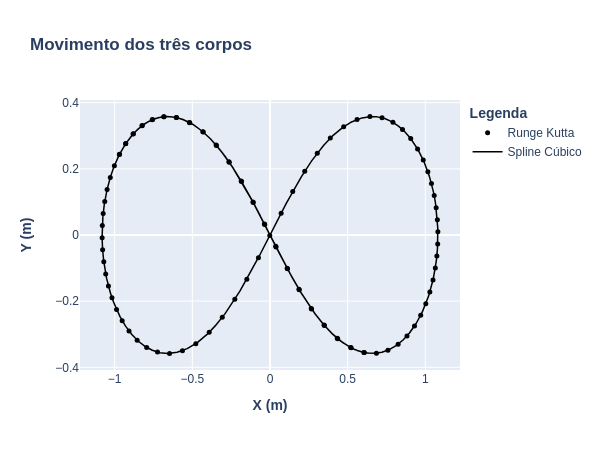
\includegraphics[width=0.9\linewidth]{SplineCubicoRK_TBP.png}
    \caption{Zoom na modelagem polinomial com splines cúbicos}
    \label{fig:enter-label}
\end{figure}


\par Respectivamente, a trajetória dos 3 planetas formando o símbolo do infinito e uma vista em escala mínima do gráfico de spline gerado por uma das trajetórias. Detalhe para a segunda imagem, onde as linhas em azul são os pontos gerados pelo Runge-Kutta e onde a linha vermelha é o spline que passa por todas os pontos. Os resultados gráficos obtidos foram extremamente satisfatórios.


\newpage
\section{Análise dos resultados}
\tab Após implementados os algoritmos em Python, como descrito na seção anterior, foi possível aproximar numericamente a solução do TBP. Para isso, problema foi discretizado com o método Runge Kutta e os pontos obtidos foram modelados com splines cúbicos, sendo que esse último método demandou técnicas de resolução de sistemas lineares para obter os coeficientes dos polinômios interpoladores.\par
Antes de apresentar os resultados e as tabelas de convergência para o TBP, é preciso verificar se os algoritmos implementados funcionam de forma ideal. Isso é necessário pois o problema do TBP é caótico e, portanto, não possui solução exata conhecida. Portanto, basta tomar um problema com solução exata conhecida, discretizá-lo com o Runge Kutta e analisar sua ordem de convergência. Tomemos, então, a seguinte igualdade:

\begin{equation}
    y = e^{3t}\cdot sen(5t) - 5
\end{equation}
\tab Assim, podemos discretizá-lo para manufaturar nosso problema:
\begin{equation}
    y' = 3e^{3t}\cdot sen(5t) + 5e^{3t}\cdot cos(5t) = f(t)
\end{equation}

\tab Definida o problema manufaturado, será preciso modificar a função de discretização utilizada no código (sem, entretanto, modificar nenhum outro trecho do algoritmo) a fim de garantir que o método utilizado converge com a ordem esperada (no caso do Runge Kutta, ordem 4).\par
Assim, dentro da classe \textit{Discretizacao}, implementamos dois novos métodos. Um deles é a função de discretização \textit{f\_manufaturada}, que recebe a variável independente \textit{t} como parâmetro e devolve o resultado descrito em (9). O outro é a solução exata \textit{exata\_manufaturada}, que possui a mesma entrada do método anterior e devolve a solução exata (8). Observe a baixo a codificação de cada um desses métodos:
\begin{lstlisting}
    def f_manufaturada(self, t): 
        """f = y' ; y = e^(3t)*sin(5t) - 5; y(0) = -5"""
        return np.exp(3*t)*3*np.sin(5*t) + 5*np.exp(3*t)*np.cos(5*t)
    
    def exata_manufaturada(self, t):
        """y = e^(3t)*sin(5t) - 5"""
        return np.exp(3*t)*np.sin(5*t) - 5
\end{lstlisting}\newpage

\tab Após executar o código \textit{main\_manufaturada.py} com o intervalo $I = [0, 2]$ com 4096 passos, obtivemos o gráfico contido na figura 4.

\begin{figure}
    \centering
    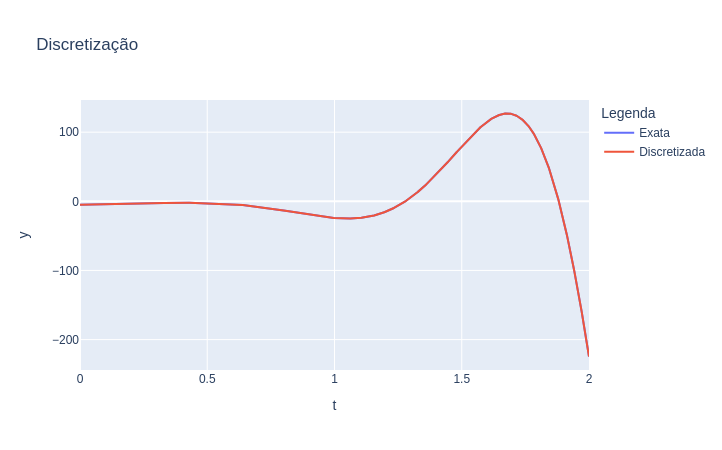
\includegraphics[width=0.9\textwidth]{DiscManufatura.png}
    \caption{Discretização do problema manufaturado com Runge Kutta}
    \label{fig:enter-label}
\end{figure}

\tab Como visto na figura, a aproximação é tão precisa que ocorre sobreposição de pixels na imagem. Somente após incrementar múltiplas vezes a escala da imagem (dentro do próprio Python com o pacote do \textit{Plotly} utilizado) é que torna-se possível observar uma mínima diferença nos pixels, o que torna o resultado obtido - sob uma primeira impressão - bastante satisfatório. \par
Além da inspeção visual do resultado, foram geradas também duas tabelas de convergência para o problema manufaturado. \par
A primeira tabela foi contruída com base na solução exata. Inicialmente, foi preciso calcular o erro $e$ das discretizações para cada número de passos $n \in [2, 4, 8, 16, 32, 64, 128, 256, 512, 1024, 2048, 4096]$. Em seguida, foi calculada a \textit{ordem $\overline{p}$ } do método. Para isso, utilizamos as seguintes expressões:
\begin{equation*}
    e(T, h_n) = |y(T) - \eta(T, h)|
\end{equation*}
\begin{equation*}    
    \log_r {\frac{e(T, h_n)}{e(T, h_{n+1)}}}
\end{equation*}
\tab Onde $r$ é a razão entre os intervalos de tempo $h$ para cada $n$ (no caso dos valores escolhidos, $r = 2$, $T$ é o instante final de tempo - ou seja, o extremo direito de I) e $\eta (T,h)$ é a aproximação numérica no instante $t = T$ com passo de tamanho $h$. Observe abaixo a tabela de convergência para o problema manufaturado:
\par
\begin{table}[!ht]
    \centering
    \begin{tabular}{|l|l|l|l|}
    \hline
        \textbf{$n$} & \textbf{$h$} & \textbf{$erro$} & \textbf{$ordem$  $\overline{p}$} \\ \hline
        2.0 & 1.0 & 84.99614863424603 & 0.0 \\ \hline
        4.0 & 0.5 & 10.853837693376335 & 2.9691922308757164 \\ \hline
        8.0 & 0.25 & 0.6506316418821143 & 4.060220443850907 \\ \hline
        16.0 & 0.125 & 0.039890889350687075 & 4.027709792859214 \\ \hline
        32.0 & 0.0625 & 0.0024801056111414255 & 4.007585826282315 \\ \hline
        64.0 & 0.03125 & 0.00015479877200164083 & 4.001935624741183 \\ \hline
        128.0 & 0.015625 & 9.67166241139239e-6 & 4.000486328281708 \\ \hline
        256.0 & 0.0078125 & 6.044279245998041e-7 & 4.000121668573305 \\ \hline
        512.0 & 0.00390625 & 3.7775862438138574e-8 & 4.000033716437231 \\ \hline
        1024.0 & 0.001953125 & 2.360991402383661e-9 & 4.0 \\ \hline
        2048.0 & 0.0009765625 & 1.4736656339664478e-10 & 4.001911660274861 \\ \hline
        4096.0 & 0.00048828125 & 9.208633855450898e-12 & 4.000278270815963 \\ \hline
    \end{tabular}
    \caption{Convergência do problema manufaturado via solução exata}
\end{table}
\tab Como esperado, temos que para números de passos progressivamente maiores, o erro converge a 0 com ordem 4. Observe que essa tabela só foi possível de ser obtida pois trata-se de um problema manufaturado, com solução exata e conhecida. Para múltiplos outros problemas, cuja solução não é conhecida (como sistemas caóticos, similares ao TBP), é preciso utilizar outra abordagem para calcular a ordem de convergência. Uma maneira de obter essa ordem é através das diferenças relativas entre aproximações sucessivamente mais refinadas. Para isso, utilizamos a seguinte expressão:
\begin{equation*}
    \overline{p} \approx \log_r {\frac{e(T, h_n)}{e(T, h_{n+1})}} = \log_r\left(\left| \frac{\eta(t, rh) - \eta(t, h)}{\eta(t, h) - \eta(t, h/r)}\right|\right)
\end{equation*}
\tab Aplicando esse método nos pontos obtidos com a solução manufaturada, obtém-se a seguinte tabela:
\newpage
\begin{table}[!ht]
    \centering


    \begin{tabular}{|l|l|l|l|}
    \hline
        \textbf{$\eta(t, 2h)$} & \textbf{$\eta(t, h)$} & \textbf{$\eta(t, h/2)$} & \textbf{$ordem$  $\overline{p}$} \\ \hline
        -139.47763176642988 & -213.61994270729957 & -223.8231487587938 & 2.8612745361219827 \\ \hline
        -213.61994270729957 & -223.8231487587938 & -224.43388951132522 & 4.062318622617734 \\ \hline
        -223.8231487587938 & -224.43388951132522 & -224.47130029506476 & 4.029034019091012 \\ \hline
        -224.43388951132522 & -224.47130029506476 & -224.4736256019039 & 4.00796118328359 \\ \hline
        -224.47130029506476 & -224.4736256019039 & -224.4737707290135 & 4.002032158043265 \\ \hline
        -224.4736256019039 & -224.4737707290135 & -224.47377979624798 & 4.000510633465523 \\ \hline
        -224.4737707290135 & -224.47377979624798 & -224.47378036290004 & 4.000127531712242 \\ \hline
        -224.47377979624798 & -224.47378036290004 & -224.47378039831491 & 4.000035964171696 \\ \hline
        -224.47378036290004 & -224.47378039831491 & -224.47378040052854 & 3.999872646001259 \\ \hline
        -224.47378039831491 & -224.47378040052854 & -224.4737804006667 & 4.002020464794127 \\ \hline
    \end{tabular}
    \caption{Convergência do problema manufaturado via diferenças relativas}
\end{table}

\tab Novamente, ainda que sem o uso da solução exata, verifica-se que o método converge a 0 com ordem 4. Importante ressaltar que enquanto o segundo método indica a proximidade entre as próprias discretizações, o primeiro revela a proximidade entre as discretizações com o resultado exato (para $h$ progressivamente refinado).
\par Aplicando, agora, os algoritmos implementados no problema dos 3 corpos, no intervalo de tempo $I = [0, 8]$ com $n \in [4, 8, 16, 32, 64, 128]$ passos, utilizando as seguintes condições iniciais:\par
\begin{table}[!ht]
    \begin{tabular}{|l|l|l|l|l|l|}
    \hline
        Corpo& $x(0)$ [m]& $y(0)$ [m]& $v_x(0)$ [m/s]&$v_y(0)$ [m/s]&Massa [Kg]\\ \hline
        1& -0.97000436& 0.24308753& 0.4662036850& 0.4323657300&1\\ \hline
        2& 0.97000436& -0.24308753& 0.4662036850& 0.4662036850&1\\ \hline
        3& 0& 0& -0.93240737& -0.86473146&1\\\hline
    \end{tabular}
    \caption{Condições inicias do TBP}
\end{table}
\tab Após gerar os pontos com as condições iniciais descritas, é possível obter uma interessante trajetória na qual os corpos movimentam-se formando o símbolo do infinito, como mostrado na figura 2. \par
Como há um grande número de variáveis no problema (6 ao todo, sendo elas a posição vertical e horizontal de cada um dos 3 corpos), optou-se por gerar um gráfico para cada uma delas a fim de facilitar a visualização, visto que a sobreposição de todos os elementos impossibilita a distinção das trajetórias para $n$ diferentes. As posições x e y de cada corpo, para múltiplos valores de $n$ se encontram nas figura 5 a 10:

\begin{figure}
    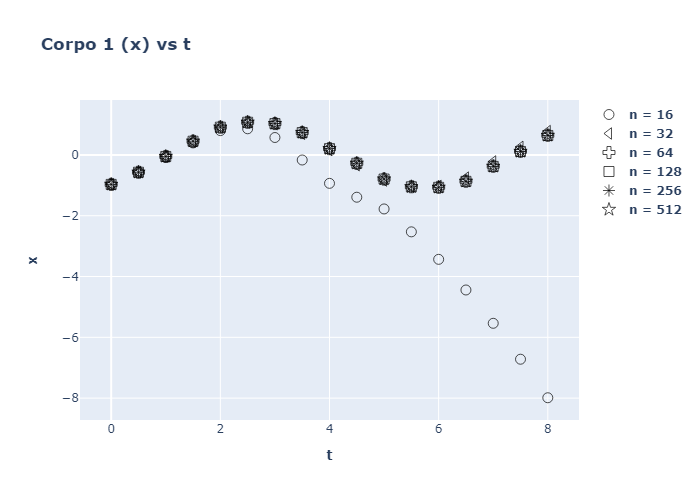
\includegraphics[width=0.75\textwidth]{Corpo1x.png}
    \caption{Discretização do TBP com Runge Kutta - Corpo 1 no eixo x}
    \label{fig:enter-label}
\end{figure}

\begin{figure}
    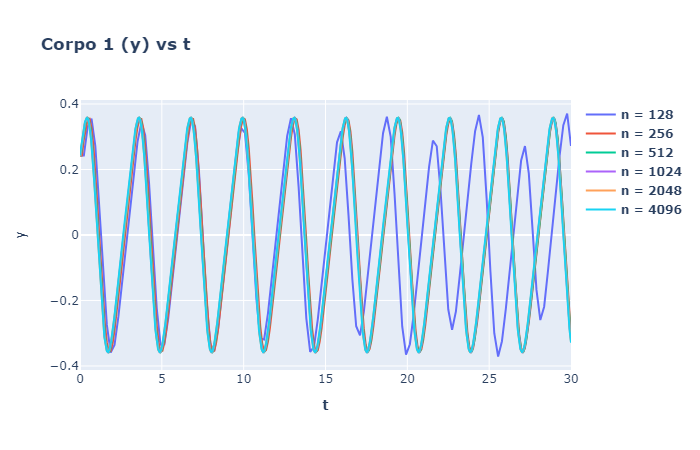
\includegraphics[width=0.75\textwidth]{Corpo1y.png}
    \caption{Discretização do TBP com Runge Kutta - Corpo 1 no eixo y}
    \label{fig:enter-label}
\end{figure}

\begin{figure}
    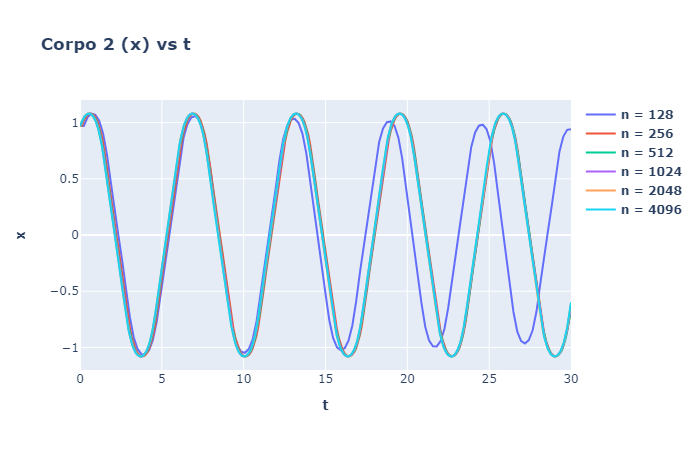
\includegraphics[width=0.75\textwidth]{Corpo2x.png}
    \caption{Discretização do TBP com Runge Kutta - Corpo 2 no eixo x}
    \label{fig:enter-label}
\end{figure}

\begin{figure}
    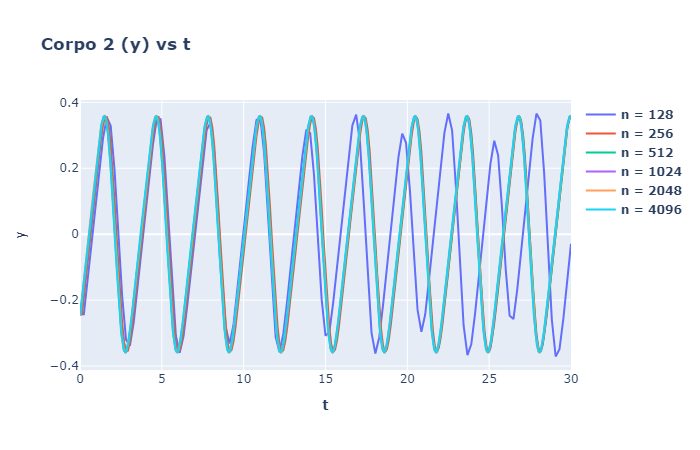
\includegraphics[width=0.75\textwidth]{Corpo2y.png}
    \caption{Discretização do TBP com Runge Kutta - Corpo 2 no eixo y}
    \label{fig:enter-label}
\end{figure}

\begin{figure}
    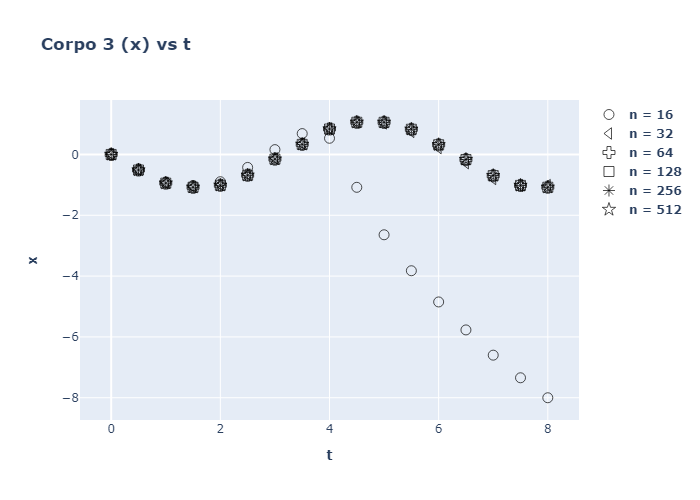
\includegraphics[width=0.75\textwidth]{Corpo3x.png}
    \caption{Discretização do TBP com Runge Kutta - Corpo 3 no eixo x}
    \label{fig:enter-label}
\end{figure}

\begin{figure}
    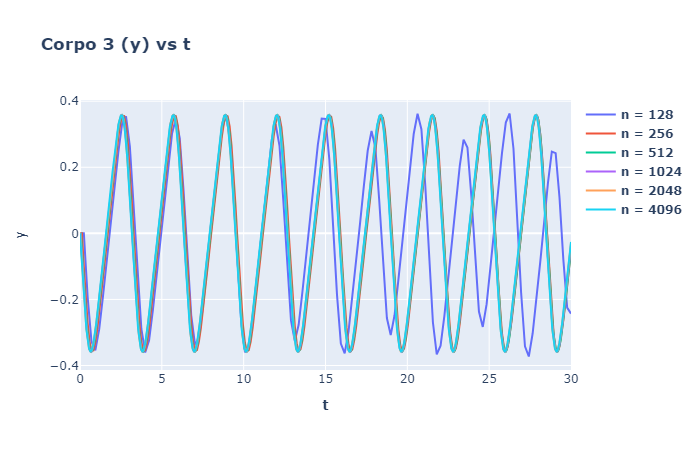
\includegraphics[width=0.75\textwidth]{Corpo3y.png}
    \caption{Discretização do TBP com Runge Kutta - Corpo 3 no eixo y}
    \label{fig:enter-label}
\end{figure}
\par
\tab Pelos gráficos, fica nítido como as trajetórias convergem para $n$ progressivamente maiores na razão 2, tendo em vista que as linhas de movimento de cada corpo começam a ficar indistinguíveis para $n > 512$. Observe, agora, as tablas de convergência via diferenças relativas para as posições $x$ e $y$ obtidas em cada corpo com o uso do Runge Kutta:

\par
\begin{table}[!ht]
    \centering
    \begin{tabular}{|l|l|l|l|l|}
    \hline
        $h$ &  $x_1(2h)$ & $x_1(h)$ & $x_1(h/2)$ & ordem $\overline{p}$ \\ \hline
        0.03125 & -7.98741 & 0.78274 & 0.64587 & 6.0017 \\ \hline
        0.01563 & 0.78274 & 0.64587 & 0.64002 & 4.54923 \\ \hline
        0.00781 & 0.64587 & 0.64002 & 0.63979 & 4.68628 \\ \hline
        0.00391 & 0.64002 & 0.63979 & 0.63978 & 4.57254 \\ \hline
    \end{tabular}
    \caption{Convergência com Runge Kutta: Corpo 1 (x)}
\end{table}

\begin{table}[!ht]
    \centering
    \begin{tabular}{|l|l|l|l|l|}
    \hline
        $h$ &  $y_1(2h)$ & $y_1(h)$ & $y_1(h/2)$ & ordem $\overline{p}$ \\ \hline
        0.03125 & 6.1181 & 0.18986 & 0.31083 & 5.6149 \\ \hline
        0.01563 & 0.18986 & 0.31083 & 0.31429 & 5.12719 \\ \hline
        0.00781 & 0.31083 & 0.31429 & 0.31442 & 4.72314 \\ \hline
        0.00391 & 0.31429 & 0.31442 & 0.31442 & 4.59087 \\ \hline
    \end{tabular}
    \caption{Convergência com Runge Kutta: Corpo 1 (y)}
\end{table}
\par
\begin{table}[!ht]
    \centering
    \begin{tabular}{|l|l|l|l|l|}
    \hline
        $h$ &  $x_2(2h)$ & $x_2(h)$ & $x_2(h/2)$ & ordem $\overline{p}$ \\ \hline
        0.03125 & -3.42258 & -0.34049 & -0.35816 & 7.44681 \\ \hline
        0.01563 & -0.34049 & -0.35816 & -0.35772 & 5.35716 \\ \hline
        0.00781 & -0.35816 & -0.35772 & -0.3577 & 3.91438 \\ \hline
        0.00391 & -0.35772 & -0.3577 & -0.35769 & 4.05073 \\ \hline
    \end{tabular}
    \caption{Convergência com Runge Kutta: Corpo 2 (x)}
\end{table}
\par
\begin{table}[!ht]
    \centering
    \begin{tabular}{|l|l|l|l|l|}
    \hline
        $h$ &  $y_2(2h)$ & $y_2(h)$ & $y_2(h/2)$ & ordem $\overline{p}$ \\ \hline
        0.03125 & -8.00064 & -1.00983 & -1.07607 & 6.72157 \\ \hline
        0.01563 & -1.00983 & -1.07607 & -1.07788 & 5.19221 \\ \hline
        0.00781 & -1.07607 & -1.07788 & -1.07795 & 4.73125 \\ \hline
        0.00391 & -1.07788 & -1.07795 & -1.07795 & 4.60167 \\ \hline
    \end{tabular}
    \caption{Convergência com Runge Kutta: Corpo 2 (y)}
\end{table}
\par
\begin{table}[!ht]
    \centering
    \begin{tabular}{|l|l|l|l|l|}
    \hline
        $h$ &  $x_3(2h)$ & $x_3(h)$ & $x_3(h/2)$ & ordem $\overline{p}$ \\ \hline
        0.03125 & 15.98805 & 0.22709 & 0.4302 & 6.27792 \\ \hline
        0.01563 & 0.22709 & 0.4302 & 0.43786 & 4.7292 \\ \hline
        0.00781 & 0.4302 & 0.43786 & 0.43816 & 4.69679 \\ \hline
        0.00391 & 0.43786 & 0.43816 & 0.43817 & 4.57922 \\ \hline
    \end{tabular}
    \caption{Convergência com Runge Kutta: Corpo 3 (x)}
\end{table}
\par
\begin{table}[!ht]
    \centering
    \begin{tabular}{|l|l|l|l|l|}
    \hline
       $h$ &  $y_3(2h)$ & $y_3(h)$ & $y_3(h/2)$ & ordem $\overline{p}$ \\ \hline
        0.03125 & -2.69552 & 0.15063 & 0.04733 & 4.78406 \\ \hline
        0.01563 & 0.15063 & 0.04733 & 0.04344 & 4.73013 \\ \hline
        0.00781 & 0.04733 & 0.04344 & 0.04328 & 4.6078 \\ \hline
        0.00391 & 0.04344 & 0.04328 & 0.04327 & 4.47808 \\ \hline
    \end{tabular}
    \caption{Convergência com Runge Kutta: Corpo 3 (y)}
\end{table}

\newpage
\tab Pelas tabelas, tal como esperado, observamos que a ordem de convergência tende a 4 (tal como no problema manufaturado). Entretanto, vale observar que, em algumas tabelas, esse valor até mesmo extrapola a ordem 4, como na tabela 7. Esse resultado pode ter ocorrido devido a natureza caótica e/ou às condições iniciais do problema. Entretanto, dado que o algoritmo do Runge Kutta utilizado foi o mesmo tanto para o problema manufaturado quanto para o TBP (alterando-se somente as condições iniciais e a função de discretização), sabemos que esse ruído no valor da ordem $\overline{p}$ não é derivado do método usado. Como forma de reiterar a validade dos programas, manufaturamos outro problema, mas agora de segunda ordem, a fim de garantir que o algoritmo funciona em problemas multidimensionais. Usamos o seguinte problema de Cauchy:
\begin{equation*}
\begin{cases}
     y''(t) = y(t) \\
    y(0) = 2 \\
    y'(0) = 3
    
\end{cases}
\end{equation*}
\par Cuja solução exata é dada por:
\begin{equation*}
    y(t) = 2,5\cdot e^t - 0,5\cdot e^{-t}
\end{equation*}
\par Assim, podemos discretizá-lo da seguinte forma:
\begin{equation*}
    \begin{cases}
        y_1(t) = y(t) \\
        y_2(t) = y_1'(t) \\
        y_2'(t) = y_1(t)
    \end{cases}
\end{equation*}
\par Com isso, obtemos os seguintes resultados:
\newpage
\begin{figure}
\centering
    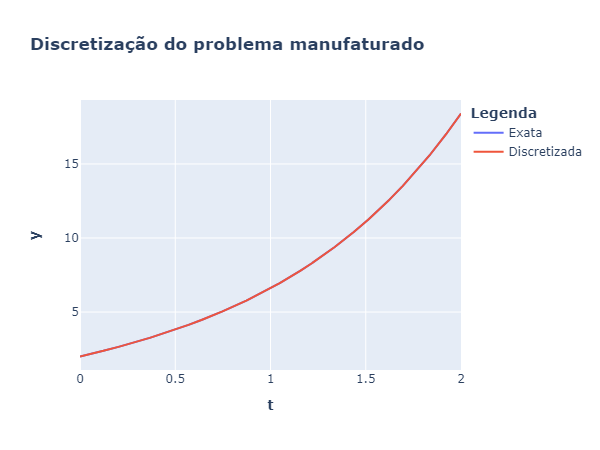
\includegraphics[width=0.75\textwidth]{DiscManufatura2.png}
    \caption{Discretização do problema manufaturado de segunda ordem com Runge Kutta}
    \label{fig:enter-label}
\end{figure}

\begin{table}[!ht]
    \centering
    \begin{tabular}{|l|l|l|l|}
    \hline
        $n$ & $h$ & erro & ordem $\overline{p}$ \\ \hline
        2.0 & 1.0 & -0.13761149459720912 & 0.0 \\ \hline
        4.0 & 0.5 & -0.012821681086780501 & 3.423943647148893 \\ \hline
        8.0 & 0.25 & -0.0009824927547299467 & 3.705994851513695 \\ \hline
        16.0 & 0.125 & -0.00006804571250285107 & 3.85187060160518 \\ \hline
        32.0 & 0.0625 & -4.477721486040309e-6 & 3.925667561154033 \\ \hline
        64.0 & 0.03125 & -2.8717390065935433e-7 & 3.9627682522515486 \\ \hline
        128.0 & 0.015625 & -1.81816766087195e-8 & 3.981367490342928 \\ \hline
        256.0 & 0.0078125 & -1.143728667329924e-9 & 3.9906685028214866 \\ \hline
        512.0 & 0.00390625 & -7.16688930424425e-11 & 3.996253952844129 \\ \hline
        1024.0 & 0.001953125 & -4.46931380793103e-12 & 4.003221820988119 \\ \hline
        2048.0 & 0.0009765625 & -3.090860900556436e-13 & 3.853972711030561 \\ \hline
    \end{tabular}
    \caption{Convergência do problema manufaturado de segunda ordem via solução exata}
\end{table}
\par
\tab Pelo gráfico e pela tabela de convergência expostos, é possível garantir, mais uma vez, que o algoritmo do Runge Kutta implementado funciona de forma correta, visto que tanto para problemas unidimensionais quanto multidimensionais - com solução exata e conhecida - o erro decai a 0 com ordem 4 para intervalos de tempo $h$ progressivamente refinados.
\par Além do método de discretização, é preciso validar tambéma implementação do spline cúbico natural. Para isso, utilizaremos duas abordagens: a primeira será comparar os resultados obtidos pelo spline com um \textit{ground true}, ou seja, uma referência científica de implementação correta (a biblioteca SciPy). Já a segunda será verificar se  


\section{Bibliografia}
A bibliografia utilizada até agora foi:
 \begin{itemize}
     \item \href{https://www.feis.unesp.br/#!/departamentos/fisica-e-quimica/grupo-de-pesquisa/gaais/grandes-cientista/johannes-kleper/}{UNESP: História de Newton}
     \item \href{https://www.feis.unesp.br/#!/departamentos/fisica-e-quimica/grupo-de-pesquisa/gaais/grandes-cientista/isaac-newton/}{UNESP: História de Kepler}
     \item \href{https://en.wikipedia.org/wiki/Three-body_problem}{Wikipedia: Three-Body Problem} 
     \item \href{https://en.wikipedia.org/wiki/Poincar%C3%A9_and_the_Three-Body_Problem}{Wikipedia: Poincaré and the Three-Body Problem}
     \item \href{https://www.google.com/search?q=simulation+three+body+problem&sca_esv=597544494&ei=lhigZeG_Ea7e1sQPvt2AmAk&udm=&oq=simulaton+of+three+bod&gs_lp=Egxnd3Mtd2l6LXNlcnAiFnNpbXVsYXRvbiBvZiB0aHJlZSBib2QqAggAMgYQABgWGB5IpLEBUOYaWI2iAXAQeACQAQSYAecBoAGpKqoBBjAuMzYuMrgBAcgBAPgBAagCCsICBxAhGAoYoAHCAgUQIRigAcICFhAAGAMYjwEY5QIY6gIYtAIYjAPYAQHCAhYQLhgDGI8BGOUCGOoCGLQCGIwD2AEBwgIIEC4YsQMYgATCAhEQLhiABBixAxiDARjHARjRA8ICCBAuGIAEGLEDwgIIEAAYgAQYsQPCAgsQABiABBixAxiDAcICDhAAGIAEGIoFGLEDGIMBwgIXEC4YsQMYgAQYlwUY3AQY3gQY4ATYAQLCAgoQABiABBiKBRhDwgIFEAAYgATCAg4QLhiABBjHARivARiOBcICCxAuGIAEGMcBGK8BwgIHEAAYgAQYCsICHRAuGIAEGMcBGK8BGI4FGJcFGNwEGN4EGOAE2AECwgITEC4YChiDARjHARixAxjRAxiABMICBRAuGIAEwgIKEAAYgAQYChixA8ICEBAAGIAEGIoFGEMYsQMYgwHCAggQLhiABBjUAsICDRAuGIAEGAoYxwEY0QPCAgkQABiABBgNGArCAgcQABiABBgNwgIHEC4YgAQYDcICCBAAGB4YDRgPwgIGEAAYHhgNwgIJEAAYgAQYDRgTwgIIEAAYHhgNGBPCAgoQABgeGA0YDxgTwgIIEAAYFhgeGBPCAgoQABgFGB4YDRgTwgIKEAAYCBgeGA0YE8ICChAAGBYYHhgTGArCAgwQABgFGB4YDRgPGBPCAgoQABgWGB4YDxgTwgIFECEYnwXiAwQYASBBiAYBugYECAEYCroGBggCEAEYFA&sclient=gws-wiz-serp#fpstate=ive&vld=cid:186afdfa,vid:cev3g826iIQ,st:0}{Material da disciplina: Three-Body Problem: A Precise Simulation}
     \item \href{https://www.wolframscience.com/reference/notes/972d/}{Stephen Wolfram, A New Kind of Science -- Notes for Chapter 7: Mechanisms in Programs and Nature; Section: Chaos Theory and Randomness from Initial Conditions}
     \item \href{https://articles.adsabs.harvard.edu/pdf/1967AJ.....72..876S}{Artigos Harvard: The Complete Solution of a General Problem of Three Bodies; Victor Szebehely and C. Frederick Peters}
     \item \href{https://plato.stanford.edu/entries/chaos/}{Stanford Encyclopedia of Philosophy -- Chaos, 2008}
     \item \href{https://cmup.fc.up.pt/cmup/relatividade/3Corpos/3corpos.html}{Oliveira, V., Cruz, I. -- O Problema dos Três Corpos}
     \item \href{https://www.sciencedirect.com/topics/mathematics/runge-kutta-method}{Método de Runge-Kutta de Discretização}
     \item \href{https://sites.icmc.usp.br/andretta/ensino/aulas/sme0500-1-12/iplagrange.pdf}{Interpolação polinomial: Polinômio de Lagrange}
     \item
     \href{https://www.ime.usp.br/mat/2458/textos/splines.pdf}{Interpolação Polinomial: Splines Cúbicos}
     \href{https://edisciplinas.usp.br/pluginfile.php/8085434/course/section/6574926/2010%20%20Burden.Faires-CHAP03.pdf}{Análise Numérica, BURDEN et al.}
 \end{itemize}


\end{document}